% Options for packages loaded elsewhere
\PassOptionsToPackage{unicode}{hyperref}
\PassOptionsToPackage{hyphens}{url}
%
\documentclass[
]{article}
\usepackage{amsmath,amssymb}
\usepackage{iftex}
\ifPDFTeX
  \usepackage[T1]{fontenc}
  \usepackage[utf8]{inputenc}
  \usepackage{textcomp} % provide euro and other symbols
\else % if luatex or xetex
  \usepackage{unicode-math} % this also loads fontspec
  \defaultfontfeatures{Scale=MatchLowercase}
  \defaultfontfeatures[\rmfamily]{Ligatures=TeX,Scale=1}
\fi
\usepackage{lmodern}
\ifPDFTeX\else
  % xetex/luatex font selection
\fi
% Use upquote if available, for straight quotes in verbatim environments
\IfFileExists{upquote.sty}{\usepackage{upquote}}{}
\IfFileExists{microtype.sty}{% use microtype if available
  \usepackage[]{microtype}
  \UseMicrotypeSet[protrusion]{basicmath} % disable protrusion for tt fonts
}{}
\makeatletter
\@ifundefined{KOMAClassName}{% if non-KOMA class
  \IfFileExists{parskip.sty}{%
    \usepackage{parskip}
  }{% else
    \setlength{\parindent}{0pt}
    \setlength{\parskip}{6pt plus 2pt minus 1pt}}
}{% if KOMA class
  \KOMAoptions{parskip=half}}
\makeatother
\usepackage{xcolor}
\usepackage[margin=1in]{geometry}
\usepackage{color}
\usepackage{fancyvrb}
\newcommand{\VerbBar}{|}
\newcommand{\VERB}{\Verb[commandchars=\\\{\}]}
\DefineVerbatimEnvironment{Highlighting}{Verbatim}{commandchars=\\\{\}}
% Add ',fontsize=\small' for more characters per line
\usepackage{framed}
\definecolor{shadecolor}{RGB}{248,248,248}
\newenvironment{Shaded}{\begin{snugshade}}{\end{snugshade}}
\newcommand{\AlertTok}[1]{\textcolor[rgb]{0.94,0.16,0.16}{#1}}
\newcommand{\AnnotationTok}[1]{\textcolor[rgb]{0.56,0.35,0.01}{\textbf{\textit{#1}}}}
\newcommand{\AttributeTok}[1]{\textcolor[rgb]{0.13,0.29,0.53}{#1}}
\newcommand{\BaseNTok}[1]{\textcolor[rgb]{0.00,0.00,0.81}{#1}}
\newcommand{\BuiltInTok}[1]{#1}
\newcommand{\CharTok}[1]{\textcolor[rgb]{0.31,0.60,0.02}{#1}}
\newcommand{\CommentTok}[1]{\textcolor[rgb]{0.56,0.35,0.01}{\textit{#1}}}
\newcommand{\CommentVarTok}[1]{\textcolor[rgb]{0.56,0.35,0.01}{\textbf{\textit{#1}}}}
\newcommand{\ConstantTok}[1]{\textcolor[rgb]{0.56,0.35,0.01}{#1}}
\newcommand{\ControlFlowTok}[1]{\textcolor[rgb]{0.13,0.29,0.53}{\textbf{#1}}}
\newcommand{\DataTypeTok}[1]{\textcolor[rgb]{0.13,0.29,0.53}{#1}}
\newcommand{\DecValTok}[1]{\textcolor[rgb]{0.00,0.00,0.81}{#1}}
\newcommand{\DocumentationTok}[1]{\textcolor[rgb]{0.56,0.35,0.01}{\textbf{\textit{#1}}}}
\newcommand{\ErrorTok}[1]{\textcolor[rgb]{0.64,0.00,0.00}{\textbf{#1}}}
\newcommand{\ExtensionTok}[1]{#1}
\newcommand{\FloatTok}[1]{\textcolor[rgb]{0.00,0.00,0.81}{#1}}
\newcommand{\FunctionTok}[1]{\textcolor[rgb]{0.13,0.29,0.53}{\textbf{#1}}}
\newcommand{\ImportTok}[1]{#1}
\newcommand{\InformationTok}[1]{\textcolor[rgb]{0.56,0.35,0.01}{\textbf{\textit{#1}}}}
\newcommand{\KeywordTok}[1]{\textcolor[rgb]{0.13,0.29,0.53}{\textbf{#1}}}
\newcommand{\NormalTok}[1]{#1}
\newcommand{\OperatorTok}[1]{\textcolor[rgb]{0.81,0.36,0.00}{\textbf{#1}}}
\newcommand{\OtherTok}[1]{\textcolor[rgb]{0.56,0.35,0.01}{#1}}
\newcommand{\PreprocessorTok}[1]{\textcolor[rgb]{0.56,0.35,0.01}{\textit{#1}}}
\newcommand{\RegionMarkerTok}[1]{#1}
\newcommand{\SpecialCharTok}[1]{\textcolor[rgb]{0.81,0.36,0.00}{\textbf{#1}}}
\newcommand{\SpecialStringTok}[1]{\textcolor[rgb]{0.31,0.60,0.02}{#1}}
\newcommand{\StringTok}[1]{\textcolor[rgb]{0.31,0.60,0.02}{#1}}
\newcommand{\VariableTok}[1]{\textcolor[rgb]{0.00,0.00,0.00}{#1}}
\newcommand{\VerbatimStringTok}[1]{\textcolor[rgb]{0.31,0.60,0.02}{#1}}
\newcommand{\WarningTok}[1]{\textcolor[rgb]{0.56,0.35,0.01}{\textbf{\textit{#1}}}}
\usepackage{graphicx}
\makeatletter
\def\maxwidth{\ifdim\Gin@nat@width>\linewidth\linewidth\else\Gin@nat@width\fi}
\def\maxheight{\ifdim\Gin@nat@height>\textheight\textheight\else\Gin@nat@height\fi}
\makeatother
% Scale images if necessary, so that they will not overflow the page
% margins by default, and it is still possible to overwrite the defaults
% using explicit options in \includegraphics[width, height, ...]{}
\setkeys{Gin}{width=\maxwidth,height=\maxheight,keepaspectratio}
% Set default figure placement to htbp
\makeatletter
\def\fps@figure{htbp}
\makeatother
\setlength{\emergencystretch}{3em} % prevent overfull lines
\providecommand{\tightlist}{%
  \setlength{\itemsep}{0pt}\setlength{\parskip}{0pt}}
\setcounter{secnumdepth}{-\maxdimen} % remove section numbering
\ifLuaTeX
  \usepackage{selnolig}  % disable illegal ligatures
\fi
\usepackage{bookmark}
\IfFileExists{xurl.sty}{\usepackage{xurl}}{} % add URL line breaks if available
\urlstyle{same}
\hypersetup{
  pdftitle={Codingchallenge7},
  pdfauthor={Samit Kafle},
  hidelinks,
  pdfcreator={LaTeX via pandoc}}

\title{Codingchallenge7}
\author{Samit Kafle}
\date{2025-04-03}

\begin{document}
\maketitle

Link to github:
\href{https://github.com/SamitKafle/coding_challenge7.git}{click here}

\textbf{1. 4 pts. Read in the data called ``PlantEmergence.csv'' using a
relative file path and load the following libraries. tidyverse, lme4,
emmeans, multcomp, and multcompView. Turn the Treatment ,
DaysAfterPlanting and Rep into factors using the function as.factor}

\begin{Shaded}
\begin{Highlighting}[]
\DocumentationTok{\#\# Load the required packages}
\FunctionTok{library}\NormalTok{(tidyverse)}
\FunctionTok{library}\NormalTok{(lme4)}
\FunctionTok{library}\NormalTok{(emmeans)}
\FunctionTok{library}\NormalTok{(multcomp)}
\FunctionTok{library}\NormalTok{(multcompView)}
\DocumentationTok{\#\# Read the data}
\NormalTok{STAND }\OtherTok{\textless{}{-}} \FunctionTok{read.csv}\NormalTok{(}\StringTok{"PlantEmergence.csv"}\NormalTok{)}

\CommentTok{\# Convert variables to factors}
\NormalTok{STAND}\SpecialCharTok{$}\NormalTok{Treatment }\OtherTok{\textless{}{-}} \FunctionTok{as.factor}\NormalTok{(STAND}\SpecialCharTok{$}\NormalTok{Treatment)}
\NormalTok{STAND}\SpecialCharTok{$}\NormalTok{DaysAfterPlanting }\OtherTok{\textless{}{-}} \FunctionTok{as.factor}\NormalTok{(STAND}\SpecialCharTok{$}\NormalTok{DaysAfterPlanting)}
\NormalTok{STAND}\SpecialCharTok{$}\NormalTok{Rep }\OtherTok{\textless{}{-}} \FunctionTok{as.factor}\NormalTok{(STAND}\SpecialCharTok{$}\NormalTok{Rep)}
\end{Highlighting}
\end{Shaded}

\textbf{2. 5 pts. Fit a linear model to predict Emergence using
Treatment and DaysAfterPlanting along with the interaction. Provide the
summary of the linear model and ANOVA results. }

\begin{Shaded}
\begin{Highlighting}[]
\CommentTok{\# Fit linear model with interaction}
\NormalTok{model\_interaction }\OtherTok{\textless{}{-}} \FunctionTok{lm}\NormalTok{(Emergence }\SpecialCharTok{\textasciitilde{}}\NormalTok{ Treatment }\SpecialCharTok{*}\NormalTok{ DaysAfterPlanting, }\AttributeTok{data =}\NormalTok{ STAND)}

\CommentTok{\# Summary and ANOVA}
\FunctionTok{summary}\NormalTok{(model\_interaction)}
\end{Highlighting}
\end{Shaded}

\begin{verbatim}
## 
## Call:
## lm(formula = Emergence ~ Treatment * DaysAfterPlanting, data = STAND)
## 
## Residuals:
##     Min      1Q  Median      3Q     Max 
## -21.250  -6.062  -0.875   6.750  21.875 
## 
## Coefficients:
##                                  Estimate Std. Error t value Pr(>|t|)    
## (Intercept)                     1.823e+02  5.324e+00  34.229   <2e-16 ***
## Treatment2                     -1.365e+02  7.530e+00 -18.128   <2e-16 ***
## Treatment3                      1.112e+01  7.530e+00   1.477    0.142    
## Treatment4                      2.500e+00  7.530e+00   0.332    0.741    
## Treatment5                      8.750e+00  7.530e+00   1.162    0.248    
## Treatment6                      7.000e+00  7.530e+00   0.930    0.355    
## Treatment7                     -1.250e-01  7.530e+00  -0.017    0.987    
## Treatment8                      9.125e+00  7.530e+00   1.212    0.228    
## Treatment9                      2.375e+00  7.530e+00   0.315    0.753    
## DaysAfterPlanting14             1.000e+01  7.530e+00   1.328    0.187    
## DaysAfterPlanting21             1.062e+01  7.530e+00   1.411    0.161    
## DaysAfterPlanting28             1.100e+01  7.530e+00   1.461    0.147    
## Treatment2:DaysAfterPlanting14  1.625e+00  1.065e+01   0.153    0.879    
## Treatment3:DaysAfterPlanting14 -2.625e+00  1.065e+01  -0.247    0.806    
## Treatment4:DaysAfterPlanting14 -6.250e-01  1.065e+01  -0.059    0.953    
## Treatment5:DaysAfterPlanting14  2.500e+00  1.065e+01   0.235    0.815    
## Treatment6:DaysAfterPlanting14  1.000e+00  1.065e+01   0.094    0.925    
## Treatment7:DaysAfterPlanting14 -2.500e+00  1.065e+01  -0.235    0.815    
## Treatment8:DaysAfterPlanting14 -2.500e+00  1.065e+01  -0.235    0.815    
## Treatment9:DaysAfterPlanting14  6.250e-01  1.065e+01   0.059    0.953    
## Treatment2:DaysAfterPlanting21  3.500e+00  1.065e+01   0.329    0.743    
## Treatment3:DaysAfterPlanting21 -1.000e+00  1.065e+01  -0.094    0.925    
## Treatment4:DaysAfterPlanting21  1.500e+00  1.065e+01   0.141    0.888    
## Treatment5:DaysAfterPlanting21  2.875e+00  1.065e+01   0.270    0.788    
## Treatment6:DaysAfterPlanting21  4.125e+00  1.065e+01   0.387    0.699    
## Treatment7:DaysAfterPlanting21 -2.125e+00  1.065e+01  -0.200    0.842    
## Treatment8:DaysAfterPlanting21 -1.500e+00  1.065e+01  -0.141    0.888    
## Treatment9:DaysAfterPlanting21 -1.250e+00  1.065e+01  -0.117    0.907    
## Treatment2:DaysAfterPlanting28  2.750e+00  1.065e+01   0.258    0.797    
## Treatment3:DaysAfterPlanting28 -1.875e+00  1.065e+01  -0.176    0.861    
## Treatment4:DaysAfterPlanting28  3.264e-13  1.065e+01   0.000    1.000    
## Treatment5:DaysAfterPlanting28  2.500e+00  1.065e+01   0.235    0.815    
## Treatment6:DaysAfterPlanting28  2.125e+00  1.065e+01   0.200    0.842    
## Treatment7:DaysAfterPlanting28 -3.625e+00  1.065e+01  -0.340    0.734    
## Treatment8:DaysAfterPlanting28 -1.500e+00  1.065e+01  -0.141    0.888    
## Treatment9:DaysAfterPlanting28 -8.750e-01  1.065e+01  -0.082    0.935    
## ---
## Signif. codes:  0 '***' 0.001 '**' 0.01 '*' 0.05 '.' 0.1 ' ' 1
## 
## Residual standard error: 10.65 on 108 degrees of freedom
## Multiple R-squared:  0.9585, Adjusted R-squared:  0.945 
## F-statistic: 71.21 on 35 and 108 DF,  p-value: < 2.2e-16
\end{verbatim}

\begin{Shaded}
\begin{Highlighting}[]
\FunctionTok{anova}\NormalTok{(model\_interaction)}
\end{Highlighting}
\end{Shaded}

\begin{verbatim}
## Analysis of Variance Table
## 
## Response: Emergence
##                              Df Sum Sq Mean Sq  F value    Pr(>F)    
## Treatment                     8 279366   34921 307.9516 < 2.2e-16 ***
## DaysAfterPlanting             3   3116    1039   9.1603 1.877e-05 ***
## Treatment:DaysAfterPlanting  24    142       6   0.0522         1    
## Residuals                   108  12247     113                       
## ---
## Signif. codes:  0 '***' 0.001 '**' 0.01 '*' 0.05 '.' 0.1 ' ' 1
\end{verbatim}

\textbf{3. 5 pts. Based on the results of the linear model in question
2, do you need to fit the interaction term? Provide a simplified linear
model without the interaction term but still testing both main effects.
Provide the summary and ANOVA results. Then, interpret the intercept and
the coefficient for Treatment 2.}

Based on the results of the linear model in Question 2, the interaction
term between Treatment and DaysAfterPlanting is not significant ( p =
1), and therefore, it can be removed

\begin{Shaded}
\begin{Highlighting}[]
\DocumentationTok{\#\# simple model}
\NormalTok{model\_simple }\OtherTok{\textless{}{-}} \FunctionTok{lm}\NormalTok{(Emergence }\SpecialCharTok{\textasciitilde{}}\NormalTok{ Treatment }\SpecialCharTok{+}\NormalTok{ DaysAfterPlanting, }\AttributeTok{data =}\NormalTok{ STAND)}
\FunctionTok{summary}\NormalTok{(model\_simple)}
\end{Highlighting}
\end{Shaded}

\begin{verbatim}
## 
## Call:
## lm(formula = Emergence ~ Treatment + DaysAfterPlanting, data = STAND)
## 
## Residuals:
##      Min       1Q   Median       3Q      Max 
## -21.1632  -6.1536  -0.8542   6.1823  21.3958 
## 
## Coefficients:
##                     Estimate Std. Error t value Pr(>|t|)    
## (Intercept)          182.163      2.797  65.136  < 2e-16 ***
## Treatment2          -134.531      3.425 -39.277  < 2e-16 ***
## Treatment3             9.750      3.425   2.847  0.00513 ** 
## Treatment4             2.719      3.425   0.794  0.42876    
## Treatment5            10.719      3.425   3.129  0.00216 ** 
## Treatment6             8.812      3.425   2.573  0.01119 *  
## Treatment7            -2.188      3.425  -0.639  0.52416    
## Treatment8             7.750      3.425   2.263  0.02529 *  
## Treatment9             2.000      3.425   0.584  0.56028    
## DaysAfterPlanting14    9.722      2.283   4.258 3.89e-05 ***
## DaysAfterPlanting21   11.306      2.283   4.951 2.21e-06 ***
## DaysAfterPlanting28   10.944      2.283   4.793 4.36e-06 ***
## ---
## Signif. codes:  0 '***' 0.001 '**' 0.01 '*' 0.05 '.' 0.1 ' ' 1
## 
## Residual standard error: 9.688 on 132 degrees of freedom
## Multiple R-squared:  0.958,  Adjusted R-squared:  0.9545 
## F-statistic: 273.6 on 11 and 132 DF,  p-value: < 2.2e-16
\end{verbatim}

\begin{Shaded}
\begin{Highlighting}[]
\FunctionTok{anova}\NormalTok{(model\_simple)}
\end{Highlighting}
\end{Shaded}

\begin{verbatim}
## Analysis of Variance Table
## 
## Response: Emergence
##                    Df Sum Sq Mean Sq F value    Pr(>F)    
## Treatment           8 279366   34921 372.070 < 2.2e-16 ***
## DaysAfterPlanting   3   3116    1039  11.068 1.575e-06 ***
## Residuals         132  12389      94                      
## ---
## Signif. codes:  0 '***' 0.001 '**' 0.01 '*' 0.05 '.' 0.1 ' ' 1
\end{verbatim}

\textbf{4. 5 pts. Calculate the least square means for Treatment using
the emmeans package and perform a Tukey separation with the compact
letter display using the cld function. Interpret the results.}

\begin{Shaded}
\begin{Highlighting}[]
\CommentTok{\# Estimate least square means}
\NormalTok{emm }\OtherTok{\textless{}{-}} \FunctionTok{emmeans}\NormalTok{(model\_simple, }\SpecialCharTok{\textasciitilde{}}\NormalTok{ Treatment)}

\CommentTok{\# Tukey }
\NormalTok{results\_lsmeans}\OtherTok{=}\FunctionTok{cld}\NormalTok{(emm, }\AttributeTok{alpha =} \FloatTok{0.05}\NormalTok{, }\AttributeTok{details=} \ConstantTok{TRUE}\NormalTok{)}
\NormalTok{results\_lsmeans}
\end{Highlighting}
\end{Shaded}

\begin{verbatim}
## $emmeans
##  Treatment emmean   SE  df lower.CL upper.CL .group
##  2           55.6 2.42 132     50.8     60.4  1    
##  7          188.0 2.42 132    183.2    192.8   2   
##  1          190.2 2.42 132    185.4    194.9   23  
##  9          192.2 2.42 132    187.4    196.9   23  
##  4          192.9 2.42 132    188.1    197.7   23  
##  8          197.9 2.42 132    193.1    202.7   23  
##  6          199.0 2.42 132    194.2    203.8    3  
##  3          199.9 2.42 132    195.1    204.7    3  
##  5          200.9 2.42 132    196.1    205.7    3  
## 
## Results are averaged over the levels of: DaysAfterPlanting 
## Confidence level used: 0.95 
## P value adjustment: tukey method for comparing a family of 9 estimates 
## significance level used: alpha = 0.05 
## NOTE: If two or more means share the same grouping symbol,
##       then we cannot show them to be different.
##       But we also did not show them to be the same. 
## 
## $comparisons
##  contrast                estimate   SE  df t.ratio p.value
##  Treatment7 - Treatment2  132.344 3.43 132  38.638  <.0001
##  Treatment1 - Treatment2  134.531 3.43 132  39.277  <.0001
##  Treatment1 - Treatment7    2.188 3.43 132   0.639  0.9993
##  Treatment9 - Treatment2  136.531 3.43 132  39.861  <.0001
##  Treatment9 - Treatment7    4.188 3.43 132   1.223  0.9502
##  Treatment9 - Treatment1    2.000 3.43 132   0.584  0.9997
##  Treatment4 - Treatment2  137.250 3.43 132  40.071  <.0001
##  Treatment4 - Treatment7    4.906 3.43 132   1.432  0.8832
##  Treatment4 - Treatment1    2.719 3.43 132   0.794  0.9969
##  Treatment4 - Treatment9    0.719 3.43 132   0.210  1.0000
##  Treatment8 - Treatment2  142.281 3.43 132  41.540  <.0001
##  Treatment8 - Treatment7    9.938 3.43 132   2.901  0.0978
##  Treatment8 - Treatment1    7.750 3.43 132   2.263  0.3724
##  Treatment8 - Treatment9    5.750 3.43 132   1.679  0.7583
##  Treatment8 - Treatment4    5.031 3.43 132   1.469  0.8678
##  Treatment6 - Treatment2  143.344 3.43 132  41.850  <.0001
##  Treatment6 - Treatment7   11.000 3.43 132   3.212  0.0425
##  Treatment6 - Treatment1    8.812 3.43 132   2.573  0.2083
##  Treatment6 - Treatment9    6.812 3.43 132   1.989  0.5538
##  Treatment6 - Treatment4    6.094 3.43 132   1.779  0.6957
##  Treatment6 - Treatment8    1.062 3.43 132   0.310  1.0000
##  Treatment3 - Treatment2  144.281 3.43 132  42.124  <.0001
##  Treatment3 - Treatment7   11.938 3.43 132   3.485  0.0187
##  Treatment3 - Treatment1    9.750 3.43 132   2.847  0.1120
##  Treatment3 - Treatment9    7.750 3.43 132   2.263  0.3724
##  Treatment3 - Treatment4    7.031 3.43 132   2.053  0.5099
##  Treatment3 - Treatment8    2.000 3.43 132   0.584  0.9997
##  Treatment3 - Treatment6    0.938 3.43 132   0.274  1.0000
##  Treatment5 - Treatment2  145.250 3.43 132  42.406  <.0001
##  Treatment5 - Treatment7   12.906 3.43 132   3.768  0.0074
##  Treatment5 - Treatment1   10.719 3.43 132   3.129  0.0535
##  Treatment5 - Treatment9    8.719 3.43 132   2.545  0.2204
##  Treatment5 - Treatment4    8.000 3.43 132   2.336  0.3288
##  Treatment5 - Treatment8    2.969 3.43 132   0.867  0.9943
##  Treatment5 - Treatment6    1.906 3.43 132   0.557  0.9998
##  Treatment5 - Treatment3    0.969 3.43 132   0.283  1.0000
## 
## Results are averaged over the levels of: DaysAfterPlanting 
## P value adjustment: tukey method for comparing a family of 9 estimates
\end{verbatim}

*Treatment 2 is significantly different from all other treatments,
having the lowest emergence (emmean = 55.6). Treatments 6, 3, and 5 had
the highest emergence (emmean ≈ 199--201) and are statistically grouped
in group 3, indicating they are significantly different from Treatment 2
and likely Treatment 7.

Treatments 1, 4, 8, and 9 fall in group ``23'', meaning they are not
significantly different from either group 2 or group 3. This suggests
intermediate performance --- not as low as Treatment 2 and not as high
as the top-performing treatments.*

\textbf{5. 4 pts. The provided function lets you dynamically add a
linear model plus one factor from that model and plots a bar chart with
letters denoting treatment differences. Use this model to generate the
plot shown below. Explain the significance of the letters. }

\begin{Shaded}
\begin{Highlighting}[]
\NormalTok{plot\_cldbars\_onefactor }\OtherTok{\textless{}{-}} \ControlFlowTok{function}\NormalTok{(lm\_model, factor) \{}
\NormalTok{  data }\OtherTok{\textless{}{-}}\NormalTok{ lm\_model}\SpecialCharTok{$}\NormalTok{model}
\NormalTok{  variables }\OtherTok{\textless{}{-}} \FunctionTok{colnames}\NormalTok{(lm\_model}\SpecialCharTok{$}\NormalTok{model)}
\NormalTok{  dependent\_var }\OtherTok{\textless{}{-}}\NormalTok{ variables[}\DecValTok{1}\NormalTok{]}
\NormalTok{  independent\_var }\OtherTok{\textless{}{-}}\NormalTok{ variables[}\DecValTok{2}\SpecialCharTok{:}\FunctionTok{length}\NormalTok{(variables)]}
  
\NormalTok{  lsmeans }\OtherTok{\textless{}{-}} \FunctionTok{emmeans}\NormalTok{(lm\_model, }\FunctionTok{as.formula}\NormalTok{(}\FunctionTok{paste}\NormalTok{(}\StringTok{"\textasciitilde{}"}\NormalTok{, factor)))}
\NormalTok{  Results\_lsmeans }\OtherTok{\textless{}{-}} \FunctionTok{cld}\NormalTok{(lsmeans, }\AttributeTok{alpha =} \FloatTok{0.05}\NormalTok{, }\AttributeTok{reversed =} \ConstantTok{TRUE}\NormalTok{, }\AttributeTok{details =} \ConstantTok{TRUE}\NormalTok{, }\AttributeTok{Letters =}\NormalTok{ letters)}
  
\NormalTok{  sig.diff.letters }\OtherTok{\textless{}{-}} \FunctionTok{data.frame}\NormalTok{(Results\_lsmeans}\SpecialCharTok{$}\NormalTok{emmeans[,}\DecValTok{1}\NormalTok{], }
                                 \FunctionTok{str\_trim}\NormalTok{(Results\_lsmeans}\SpecialCharTok{$}\NormalTok{emmeans[,}\DecValTok{7}\NormalTok{]))}
  \FunctionTok{colnames}\NormalTok{(sig.diff.letters) }\OtherTok{\textless{}{-}} \FunctionTok{c}\NormalTok{(factor, }\StringTok{"Letters"}\NormalTok{)}
  
\NormalTok{  ave\_stand2 }\OtherTok{\textless{}{-}}\NormalTok{ lm\_model}\SpecialCharTok{$}\NormalTok{model }\SpecialCharTok{\%\textgreater{}\%}
    \FunctionTok{group\_by}\NormalTok{(}\SpecialCharTok{!!}\FunctionTok{sym}\NormalTok{(factor)) }\SpecialCharTok{\%\textgreater{}\%}
\NormalTok{    dplyr}\SpecialCharTok{::}\FunctionTok{summarize}\NormalTok{(}
      \AttributeTok{ave.emerge =} \FunctionTok{mean}\NormalTok{(.data[[dependent\_var]], }\AttributeTok{na.rm =} \ConstantTok{TRUE}\NormalTok{),}
      \AttributeTok{se =} \FunctionTok{sd}\NormalTok{(.data[[dependent\_var]]) }\SpecialCharTok{/} \FunctionTok{sqrt}\NormalTok{(}\FunctionTok{n}\NormalTok{())}
\NormalTok{    ) }\SpecialCharTok{\%\textgreater{}\%}
    \FunctionTok{left\_join}\NormalTok{(sig.diff.letters, }\AttributeTok{by =}\NormalTok{ factor) }\SpecialCharTok{\%\textgreater{}\%}
    \FunctionTok{mutate}\NormalTok{(}\AttributeTok{letter\_position =}\NormalTok{ ave.emerge }\SpecialCharTok{+} \DecValTok{10} \SpecialCharTok{*}\NormalTok{ se)}
  
\NormalTok{  plot }\OtherTok{\textless{}{-}} \FunctionTok{ggplot}\NormalTok{(data, }\FunctionTok{aes}\NormalTok{(}\AttributeTok{x =} \SpecialCharTok{!!} \FunctionTok{sym}\NormalTok{(factor), }\AttributeTok{y =} \SpecialCharTok{!!} \FunctionTok{sym}\NormalTok{(dependent\_var))) }\SpecialCharTok{+} 
    \FunctionTok{stat\_summary}\NormalTok{(}\AttributeTok{fun =}\NormalTok{ mean, }\AttributeTok{geom =} \StringTok{"bar"}\NormalTok{) }\SpecialCharTok{+}
    \FunctionTok{stat\_summary}\NormalTok{(}\AttributeTok{fun.data =}\NormalTok{ mean\_se, }\AttributeTok{geom =} \StringTok{"errorbar"}\NormalTok{, }\AttributeTok{width =} \FloatTok{0.5}\NormalTok{) }\SpecialCharTok{+}
    \FunctionTok{ylab}\NormalTok{(}\StringTok{"Number of emerged plants"}\NormalTok{) }\SpecialCharTok{+} 
    \FunctionTok{geom\_jitter}\NormalTok{(}\AttributeTok{width =} \FloatTok{0.02}\NormalTok{, }\AttributeTok{alpha =} \FloatTok{0.5}\NormalTok{) }\SpecialCharTok{+}
    \FunctionTok{geom\_text}\NormalTok{(}\AttributeTok{data =}\NormalTok{ ave\_stand2, }\FunctionTok{aes}\NormalTok{(}\AttributeTok{label =}\NormalTok{ Letters, }\AttributeTok{y =}\NormalTok{ letter\_position), }\AttributeTok{size =} \DecValTok{5}\NormalTok{) }\SpecialCharTok{+}
    \FunctionTok{xlab}\NormalTok{(}\FunctionTok{as.character}\NormalTok{(factor)) }\SpecialCharTok{+}
    \FunctionTok{theme\_classic}\NormalTok{()}
  
  \FunctionTok{return}\NormalTok{(plot)}
\NormalTok{\}}

\CommentTok{\# Example usage}
\FunctionTok{plot\_cldbars\_onefactor}\NormalTok{(model\_simple, }\StringTok{"Treatment"}\NormalTok{)}
\end{Highlighting}
\end{Shaded}

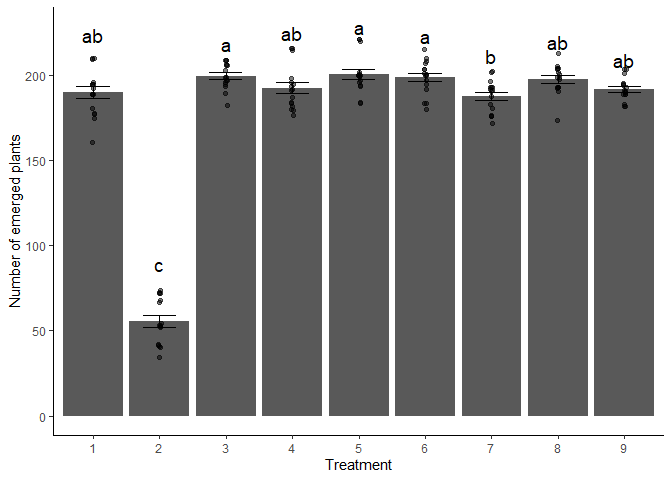
\includegraphics{codingchallenge7_files/figure-latex/unnamed-chunk-5-1.pdf}

\emph{Treatments sharing the same letter are not significantly
different. Treatment 2 (group ``c'') had significantly lower emergence
than all others. Treatments 3, 5, and 6 (group ``a'') had the highest
emergence and are not significantly different from each other.
Treatments labeled ``ab'' (1, 4, 8, 9) are not significantly different
from either group ``a'' or ``b''}

\end{document}
